\chapter{Analytical Solutions}
\label{lec:analytical}

In this lecture, we analyze the neutron transport equation analytically for several simple cases.  In particular, we investigate neutron streaming in a vacuum and in a purely absorbing slab.  The next lecture offers further analytical and semi-analytical treatments using the integral form of the transport equation.  These two lectures ultimately show the difficulty with which realistic problems can be addressed by ``pen and paper'' and serve to motivate our later discussions of deterministic numerical methods.

\section*{One-Speed Transport}

Before we consider solutions to the transport equation, we first eliminate the energy dependence.  The reason for this is simple: \textit{the energy is simply too hard to deal with directly}.  The dependence of the various cross-sections on the energy is erratic, and, as we have seen in previous lectures, there are isotopes whose dependence on energy in certain energy ranges cannot even be resolved!

We can eliminate $E$ in two ways.  First, we can assume that $\psi$ and the cross-sections are constant in energy within an energy range $E_g < E < E_{g-1}$; this is the multi-group method, which has been the workhorse of deterministic transport methods for decades\footnote{A new methodology being developed here at MIT is a generalization of the multigroup method where instead of flat fluxes within groups (a ``zeroth`` order representation), the fluxes can have higher order dependences (linear, parabolic, etc.) using discrete Legendre polynomial expansions.}.  A second, somewhat superficial approach is to multiply the energy-dependent transport equation by $\delta(E-E_0)$.   Since $f(x)\delta(x-x_0) = f(x_0)$, we have for $E_0$ (or a groups $g$) the time- and energy-independent or \textit{one-speed transport equation}:
\begin{equation}
     \hat{\Omega} \cdot \nabla \psi(\mathbf{r},\mathbf{\Omega})  + \Sigma_t \psi(\mathbf{r},\mathbf{\Omega}) =   \int_{4\pi} d\Omega' \Sigma_s(\mathbf{r},\mathbf{\Omega}\cdot\mathbf{\Omega}')\psi(\mathbf{r},\mathbf{\Omega'}) + s(\mathbf{r},\mathbf{\Omega})  \, .
\end{equation}

\section*{Streaming in Vacuum}

Perhaps the easiest class of problems to consider are those whose medium is vacuum.  In this case, there are no particle interactions, and all we need to do is follow particles along trajectories from sources.  These trajectories are called \textit{characteristics}, and in general, the \textit{method of characteristics} is the mathematical technique we can use to find $\psi$.  Note, a more general use of the \textit{method of characteristics} applies to arbitrary media and is fast becoming the standard transport method in lattice physics.

\section*{The Streaming Term}

Consider the streaming of neutrons in a sourceless vacuum:
\begin{equation}
     \hat{\Omega} \cdot \nabla \psi(\mathbf{r},\mathbf{\Omega}) =   0  \, .
\end{equation}
What form does the streaming term $ \hat{\Omega} \cdot \nabla \psi $ have?  It depends crucially on the underlying coordinate systems.  

It helps to note that  $\mathbf{\hat{\Omega}} \cdot \nabla \psi$ is just the spatial rate of change of $\psi$ along the direction of travel, i.e. along the characteristic.  Suppose we have a particle originally at a location $\mathbf{r}_0$  going in a direction $\mathbf{\Omega}$.  Then upon traveling a distance $s$, the location $\mathbf{r} = \mathbf{r}_0 + s\mathbf{\Omega}$.  Accordingly, the spatial rate of change of $\psi$ can be written
\begin{equation}
    \frac{d}{ds} \psi(\mathbf{r}_0 +s\mathbf{\Omega},\mathbf{\Omega}) =   0  \, .
    \label{eq:spaceratepsi}
\end{equation}

We can also show more explicitly that $\frac{d\psi}{ds} = \hat{\Omega} \cdot \nabla \psi$.  In general, the direction vector $\mathbf{\Omega}$ has the basic form
\begin{equation}
 \mathbf{\Omega} = \mu \mathbf{\hat{e}}_{\mu} + \eta \mathbf{\hat{e}}_{\eta} + \xi \mathbf{\hat{e}}_{\xi} \, ,
\end{equation}
where $\mu$, $\eta$, and $\xi$ are directional cosines and the $\mathbf{\hat{e}}$'s are corresponding coordinate vectors.  In general, $\mathbf{\Omega}$ depends on three spatial coordinates $p_1$, $p_2$, and $p_3$ and two angular coordinates, usually parameterized as the cosine of the polar angle $\chi = \cos(\theta)$\footnote{We use $\chi$ to represent the polar angle cosine in general rather than $\mu$, since $\mu$ here will be the directional cosine with respect to the $x$ axis.} and the azimuthal angle $\phi$.  Hence,
\begin{equation}
 \frac{d}{ds} = \frac{dp_1}{ds}\frac{\partial}{\partial p_1} + \frac{dp_2}{ds}\frac{\partial}{\partial p_2} + \frac{dp_3}{ds}\frac{\partial}{\partial p_3} + \frac{d\mu}{ds}\frac{\partial}{\partial \mu} + \frac{d\phi}{ds}\frac{\partial}{\partial \phi} \, .
 \label{eq:totalsderivative}
\end{equation}
The various derivatives in Eq. \ref{eq:totalsderivative} may or may not vanish, depending on the geometry.  Consider Cartesian geometry where $p_1 = x$ and so on.  The Cartesian spatial and angular system was given in Figure \ref{fig:phase_space}, where the polar angle was defined with respect to the $z$ axis and the azimuth with respect to the $x$ axis.  Any incremental movement $ds$ along the direction $\mathbf{\Omega}$ can be seen  to change neither $\theta$ (nor its cosine $\xi$) nor $\phi$, since the angular coordinate system is invariant as the particle moves.  All this means is that $\mathbf{\Omega}$ at $\mathbf{r}_0$ is the same as the $\mathbf{\Omega}$ at $\mathbf{r}_0 + ds\mathbf{\Omega}$.  Hence, $d\xi/ds = d\phi/ds = 0$ and
\begin{equation}
 \frac{d}{ds} = \frac{dx}{ds}\frac{\partial}{\partial x} + \frac{dy}{ds}\frac{\partial}{\partial y} + \frac{dz}{ds}\frac{\partial}{\partial z} \, ,
\end{equation}
but $dx/ds$ is just the directional cosine with respect to the $x$ axis, $\mu$, and likewise $dx/ds = \eta$ and $dz/ds = \xi$ so that
\begin{equation}
 \frac{d}{ds} = \mu \frac{\partial}{\partial x} + \eta \frac{\partial}{\partial y} + \xi \frac{\partial}{\partial z} = \mathbf{\Omega} \cdot \nabla  \, .
\end{equation}

For other geometries, the streaming term is not as simple, since the angular coordinate system does depend on the position $\mathbf{r}$.  The spherical spatial and angular system is given if Figure \ref{fig:spherical_phase_space}.  The three spatial coordinates are $r$, $\theta_r$ and $\phi_r$.  The angular coordinate system is such that the polar angle is defined with respect to $\mathbf{r}$.  The azimuth and secondary coordinates are defined somewhat arbitrarily.

\begin{figure}[ht] 
    \centering
    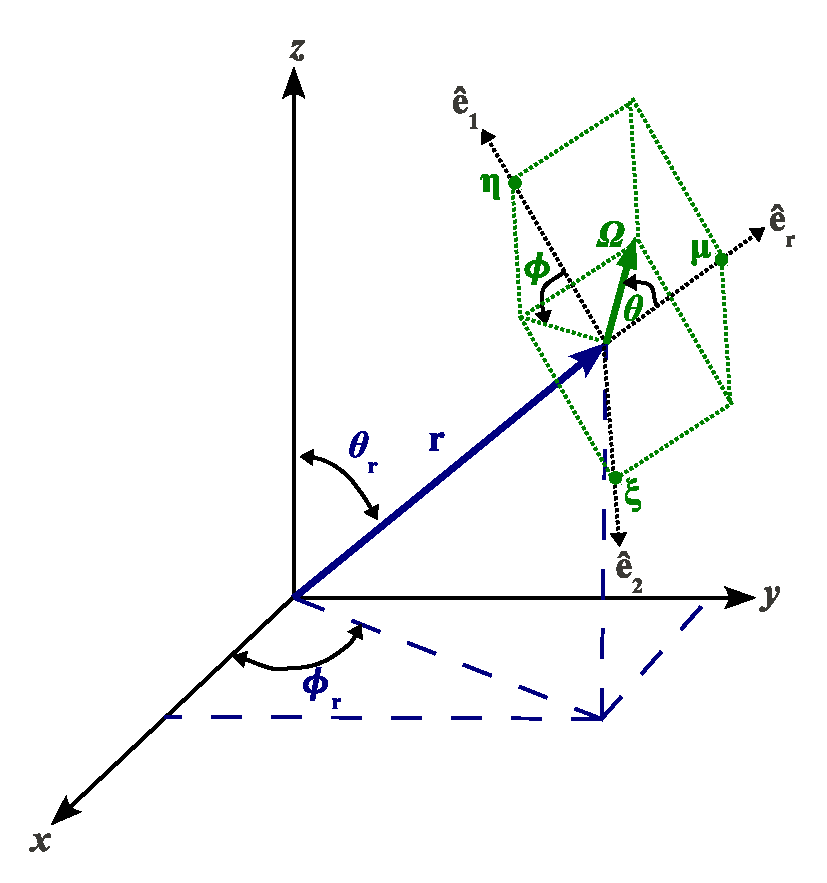
\includegraphics[keepaspectratio, width = 3.0 in]{images/spherical_phase_space}
    \caption{Spherical phase space.}
    \label{fig:spherical_phase_space}
\end{figure}

The streaming operator in spherical coordinates is defined generally as 
\begin{equation}
 \frac{d}{ds} = \frac{dr}{ds}\frac{\partial}{\partial r} + \frac{d\theta_r}{ds}\frac{\partial}{\partial \theta_r} + \frac{d\phi_r}{ds}\frac{\partial}{\partial \phi_r} + \frac{d\mu}{ds}\frac{\partial}{\partial \mu} + \frac{d\phi}{ds}\frac{\partial}{\partial \phi} \, .
\end{equation}
As a simple example, consider the case of 1-d transport in spherical coordinates, for which we assume the flux is independent of the spatial coordinates $\theta_{r}$ and $\phi_{r}$, which eliminates the derivatives with respect to $\theta_r$ and $\phi_r$.  Moreover, if we look at the angular coordinates, we see that if $r$ is the only spatial variable, then there should be dependence only on $\mu$.  A dependence on the azimuthal angle would require a non-uniform particle distribution in the other spatial directions.  Hence, the derivative with respect to $\phi$ also vanishes, leaving
\begin{equation}
 \frac{d}{ds} = \frac{dr}{ds}\frac{\partial}{\partial r} + \frac{d\mu}{ds}\frac{\partial}{\partial \mu}  \, .
\end{equation}
From Figure \ref{fig:spherical_phase_space}, we can immediately see that
\begin{equation}
 \frac{dr}{ds} = \mu \, .
 \label{eq:drds}
\end{equation}
Less obvious is $d\mu/ds$.  First note that $r d\theta = -ds \sin\theta$, which we can see directly from Figure \ref{fig:spherical_angle_with_r}.  The negative sign arises because a positive $ds$ leads to a decrease $\theta$. Then, noting that $\mu = \cos{\theta}$ so that $d\mu = -\sin{\theta} d\theta$, we can show
\begin{equation}
 \frac{d\mu}{ds} = \frac{1-\mu^2}{r} \, ,
 \label{eq:dmuds}
\end{equation}
and
\begin{equation}
 \frac{d\psi}{ds} = \mathbf{\Omega} \cdot \nabla_{\text{1d}} \psi = \mu \frac{\partial \psi}{\partial r} \frac{1-\mu^2}{r}\frac{\partial \psi}{\partial \mu} \, .
\end{equation}


\begin{figure}[ht] 
    \centering
    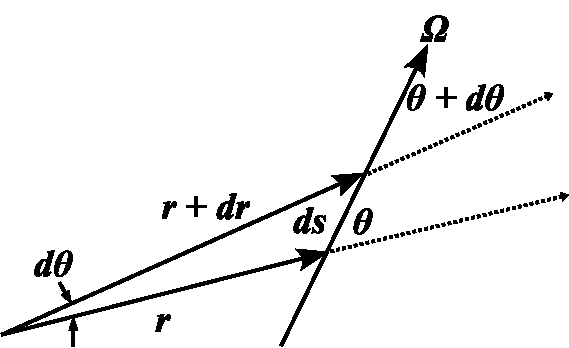
\includegraphics[keepaspectratio, width = 2.5 in]{images/spherical_angle_with_r}
    \caption{Change in $r$ and $\theta$ as a particle streams.}
    \label{fig:spherical_angle_with_r}
\end{figure}


\section*{Example 1: Meandering from a Plane Source in a Vacuum Slab}

As a first example, consider the case of neutrons streaming in a 1-d slab for $x>0$ where the source is an isotropic planar source at $x=0$ which we will use as a boundary condition rather than a source term. The Cartesian streaming term above simplifies in 1-d to
\begin{equation}
 \mu \frac{\partial \psi}{\partial x} = 0 \, ,
\end{equation}
subject to
\begin{equation}
 \psi(0,\mu) = \frac{S_0}{2} \, .
\end{equation}
In 1-d slab geometry, we essentially integrate out the 2$\pi$ associated with the azimuthal angle.  Hence, isotropic sources of strength $S$ become $S/2$ instead of $S/4\pi$.  The units of $\psi$ are slightly different, and one must divide by $2\pi$ [rad] in order to obtain units appropriate in 3-d.  Integrating the equations shows that
\begin{equation}
 \psi(x,\mu) = c \, , \, \, \, \, \mu > 0 \, ,
\end{equation}
for some constant $c$.  At $x = 0$, we must have $\psi(0,\mu) = S/2$, and so for all $x > 0$, $\psi(x,\mu) = S/2$.  The same hold for negative $x$ and $\mu$.

\section*{Example 2: Playing in Vacuum Outside a Spherical Shell Source}

We now consider a neutrons streaming in a vacuum due to an isotropic spherical shell source of radius $r_0$.  We focus only on $r > r_0$.  The transport equation can be written
\begin{equation}
 \mu \frac{\partial \psi}{\partial r} + \frac{1-\mu^2}{r} \frac{\partial \psi}{\partial \mu} = \frac{S_0\delta(r-r_0)}{4\pi r_0} \, .
\end{equation}
From Eqs. \ref{eq:drds} and \ref{eq:dmuds}, we have
\begin{equation}
 ds = \frac{d\mu}{ (1-\mu^2)/r } = \frac{dr}{\mu} \, ,
\end{equation}
or
\begin{equation}
 \frac{dr}{r} = \frac{\mu d\mu}{1-\mu^2} \, .
\end{equation}
We integrate from initial coordinates $r_s$ and $\mu_s$, as shown in Figure \ref{fig:sphere_example}, and rearrange to obtain
\begin{equation}
 \mu = \sqrt{ 1 - (1-\mu^2_s)\Big (\frac{r_s}{r} \Big )^2  } \, .
 \label{eq:angularrestribution}
\end{equation}
\begin{figure}[ht] 
    \centering
    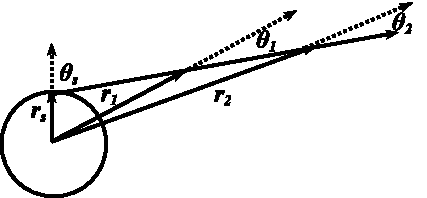
\includegraphics[keepaspectratio, width = 2.5 in]{images/sphere_example}
    \caption{Streaming of particles from spherical shell source.}
    \label{fig:sphere_example}
\end{figure}

Eq. \ref{eq:angularrestribution} shows explicitly how $\mu$ changes as a function of $r$.  This phenomenon is often called angular redistribution and leads to collimation of the flux away from the source.  Since $d\psi/ds$ must equal the source, we can write
\begin{equation}
 ds = \frac{d\mu}{ (1-\mu^2)/r } = \frac{d\psi}{ \frac{S_0\delta(r-r_0)}{4\pi r_0}  } \, ,
\end{equation}
or 
\begin{equation}
\frac{d\psi}{dr} = \frac{S_0\delta(r-r_0)}{4\pi r_0} \, .
\end{equation}
Then
\begin{equation}
 \int^{r,\mu}_{r_s,\mu_s} \frac{d\psi}{dr}  = \int^r_{r_s} dr \frac{S_0\delta(r-r_0)}{4\pi r_0} \, ,
\end{equation}
or
\begin{equation}
 \psi(r,\mu)-\psi(r_s,\mu_s) = \frac{S_0}{8\pi r^2_s} \frac{1}{\sqrt{1-(1-\mu^2_s)}} \, .
\end{equation}
We take the boundary flux to be $\psi(r_s,\mu_s) = 0$, which implies that $\mu_s$ is limited to $\mu_s \leq 0 \leq \pi/2$. If $\mu_s$ spanned through $\pi$, then particles could be born into the sphere and stream out of another location, a complication we care to avoid in this example.  From Eq. \ref{eq:angularrestribution}, we have $(1-\mu^2_s)=(r/r_s)^2(1-\mu^2)$.  We note that for $\mu_s = 0$, $\mu=\sqrt{1-(r_s/r)^2}$ and when $\mu_s=1$, $\mu=1$.  Finally, we have
\begin{equation}
 \psi(r,\mu) = \frac{S_0}{8\pi} \frac{1}{\sqrt{r^2_s - r^2(1-\mu^2)}} \, , \, \, \, \, \, \sqrt{1-\Big ( \frac{r_s}{r} \Big )^2 } \leq \mu \leq 1 \, .
 \label{eq:spherepsi}
\end{equation}

To illustrate the behavior of $\psi$, we have taken $r_s = 1$ and $S_0 = 8\pi$.  Figure \ref{fig:sphere_psi_radius} shows $\psi$ as a function of radius for several $\mu$ values.  Of course, we see that as neutrons move farther from the source, the flux at larger $\theta$ values (smaller $\mu$ values) diminishes, as we expect due to angular redistribution. Figure \ref{fig:sphere_psi_mu} shows $\psi$ as a function of $\mu$ for several values of $r$.  We see effects of the same phenomenon, in that the angular distribution becomes more collimated about $\mu = 1$ for larger $r$.
\begin{figure}[ht] 
    \centering
    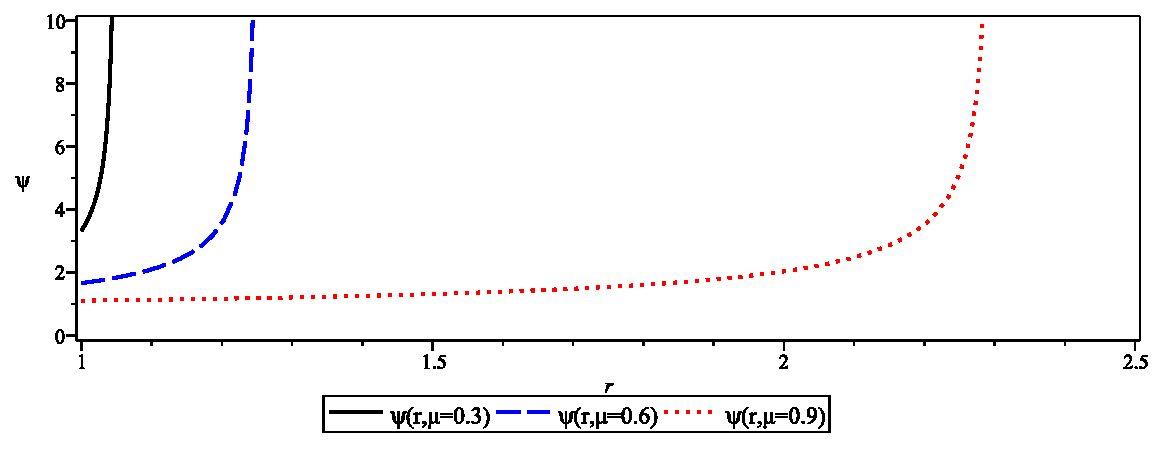
\includegraphics[keepaspectratio, width = 5.0 in]{images/sphere_psi_radius}
    \caption{Angular flux as a function of radius for certain $\mu$ values.}
    \label{fig:sphere_psi_radius}
\end{figure}

\begin{figure}[ht] 
    \centering
    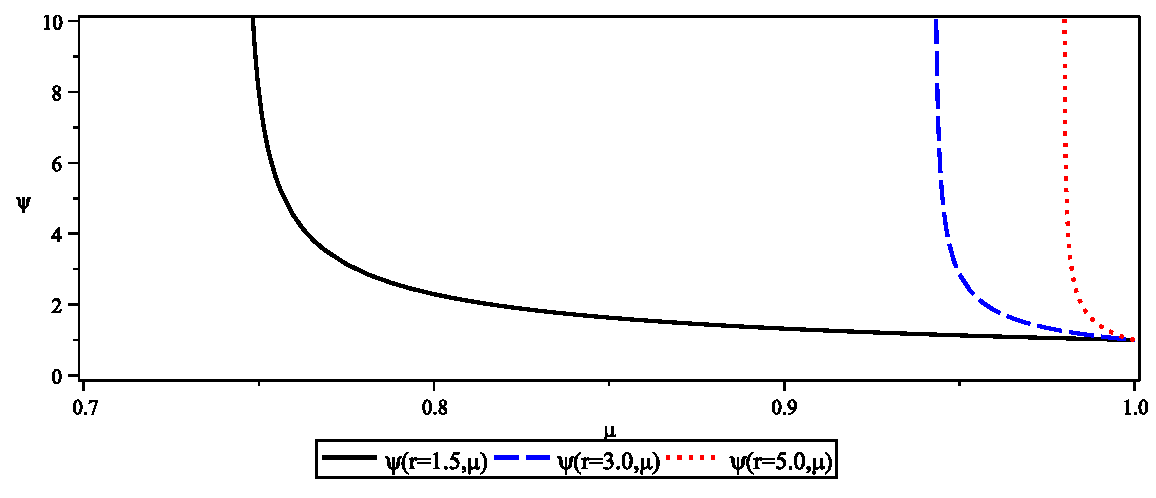
\includegraphics[keepaspectratio, width = 5.0 in]{images/sphere_psi_mu}
    \caption{Angular flux as a function of $\mu$ at certain $r$ values.}
    \label{fig:sphere_psi_mu}
\end{figure}

\section*{Example 3: A Purely Absorbing Slab}

As a final example, we apply what we've learned in vacuum to transport in a purely absorbing slab.  In this case, the 1-d transport equation is
\begin{equation}
 \mu \frac{\partial \psi}{\partial x} + \Sigma_a(x)\psi(x,\mu) = S(x,\mu) \, .
\end{equation}
As an example, we study a uniform slab of length $L$, subject to vacuum boundaries, and with a uniform, isotropic source of volumetric strength\footnote{By volumetric strength, we mean the units are neutrons per unit volume per second.} $S_0$.  Our equation simplifies to 
\begin{equation}
 \mu \frac{\partial \psi}{\partial x} + \Sigma_a \psi(x,\mu) = \frac{S_0}{2} \, .
 \label{eq:slababsorber}
\end{equation}
To solve the problem, we decompose $\psi$ into $\psi_+$ for $\mu > 0$ and $\psi_-$ for $\mu < 0$.  In this way, we can start at one end of the slab and work our way across, essentially as would a neutron.

For $\mu>0$, we divide Eq. \ref{eq:slababsorber} through by $\mu$ and compute the integrating factor
\begin{equation}
 if = \exp{\int^x_0 dx \Sigma_a\mu} = \exp{\Sigma_a x/\mu} \, .
\end{equation}
Then we have
\begin{equation}
 \frac{d}{dx}\Big ( \psi_{+} e^{\Sigma_a x} \Big ) = \frac{S_0}{2\mu}  e^{\Sigma_a x/\mu} \, ,
\end{equation}
and integrating from $0$ to $x$ yields
\begin{equation}
 \psi_{+} = \frac{S_0}{2\Sigma_a}\Bigg (1 - e^{-\Sigma_a x/\mu} \Bigg ) \, ,
\end{equation}
where we note $\psi_+{0,\mu} = 0$ from the given boundary condition.

For $\mu<0$, we do similarly.  It helps in this case to use $-|\mu|$ in place of $\mu$, as it can be easy to lose negative signs.  Using the integrating factor $\exp{(L-x)/|\mu|}$, we find after integrating from $L$ to $x$ that
\begin{equation}
 \psi_{-} = \frac{S_0}{2\Sigma_a}\Bigg (1 - e^{-\Sigma_a (L-x)/|\mu|} \Bigg ) \, .
\end{equation}
For the case of $L = 10$ and $\Sigma_a = 1$, Figure \ref{fig:slab_example_psi} shows $\psi$ for several values of $\psi$.  Note the symmetry, as should be expected. 

\begin{figure}[ht] 
    \centering
    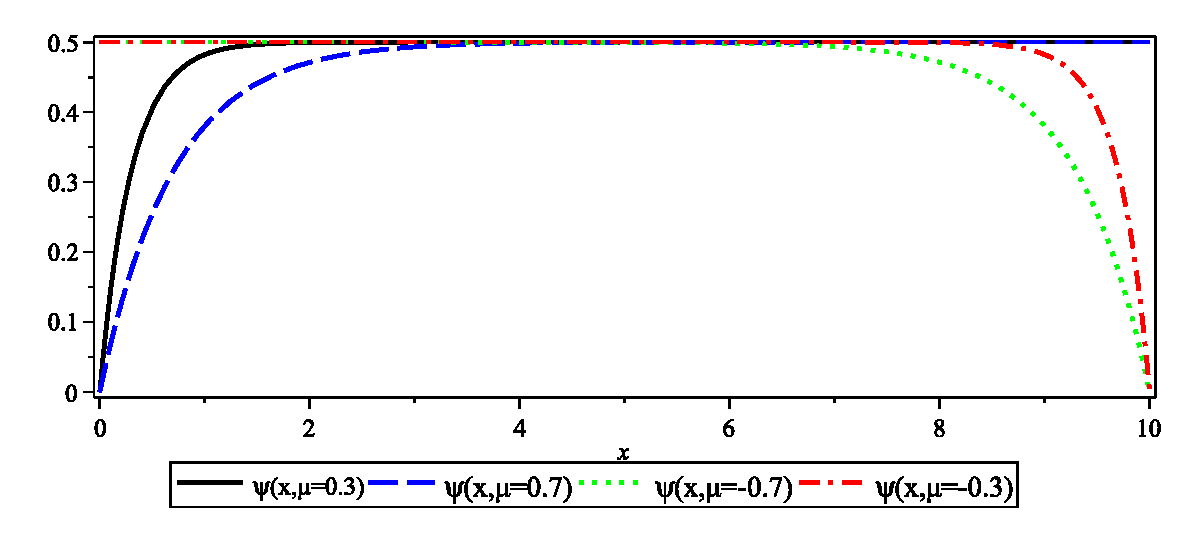
\includegraphics[keepaspectratio, width = 5.0 in]{images/slab_example_psi}
    \caption{Angular flux at specific angles for the absorbing slab.}
    \label{fig:slab_example_psi}
\end{figure}

Our next goal is to compute the scalar flux.  By definition, the scalar flux in 1-d is
\begin{equation}
 \phi(x) = \int^1_{-1} d\mu \psi(x,\mu) \, ,
\end{equation}
which can be broken into
\begin{equation}
  \phi(x) = \int^0_{-1} d\mu \psi_{-}(x,\mu) + \int^1_{0} d\mu \psi_{+}(x,\mu) \, .
\end{equation}
Inserting our expressions above, we have
\begin{equation}
\begin{split}
  \phi(x) &= \frac{S_0}{2\Sigma_a} \Bigg (  \int^{1}_{-1} d\mu - \int^0_{-1} d\mu  e^{-\Sigma_a (L-x)/|\mu|} - \int^1_{0} d\mu e^{-\Sigma_a x/\mu}  \Bigg ) \\
          &= \frac{S_0}{2\Sigma_a} \Bigg ( 2 - \int^1_{0} d\mu'  e^{-\Sigma_a (L-x)/\mu} - \int^1_{0} d\mu e^{-\Sigma_a x/\mu}  \Bigg ) \\
          &= \frac{S_0}{2\Sigma_a} \Bigg ( 2 - E_2(\Sigma_a (L-x)) - E_2(\Sigma_a x)  \Bigg ) \, .
\end{split}
\end{equation}
For the same numerical example, $\phi(x)$ is shown if Figure \ref{fig:slab_example_phi_current} along with the current density $\mathbf{J}(x)$, computation of which is left as an exercise.

\begin{figure}[ht] 
    \centering
    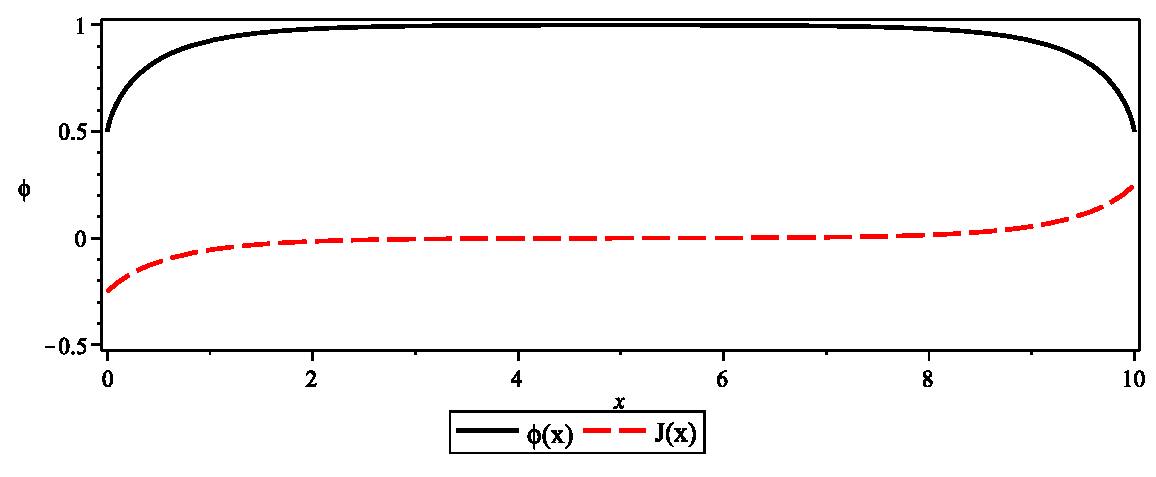
\includegraphics[keepaspectratio, width = 5.0 in]{images/slab_example_phi_current}
    \caption{Scalar flux and current density.}
    \label{fig:slab_example_phi_current}
\end{figure}

\section*{Exponential Integrals}

The functions $E_n(x)$ are called ``exponential integrals'' and are characteristic of slab problems.  They are defined by
\begin{equation}
 E_n(x) \equiv \int^1_0 d\mu \mu^{n-2} e^{-x/\mu} \, .
 \label{eq:EnDefinition}
\end{equation}
They also satisfy
\begin{equation}
 E_n(x) = - \int dx E_{n-1}(x) \, .
 \label{eq:EnIntegration}
\end{equation}
Several of the $E_n$ functions are shown in Figure \ref{fig:slab_example_exp_functions}.

\begin{figure}[ht] 
    \centering
    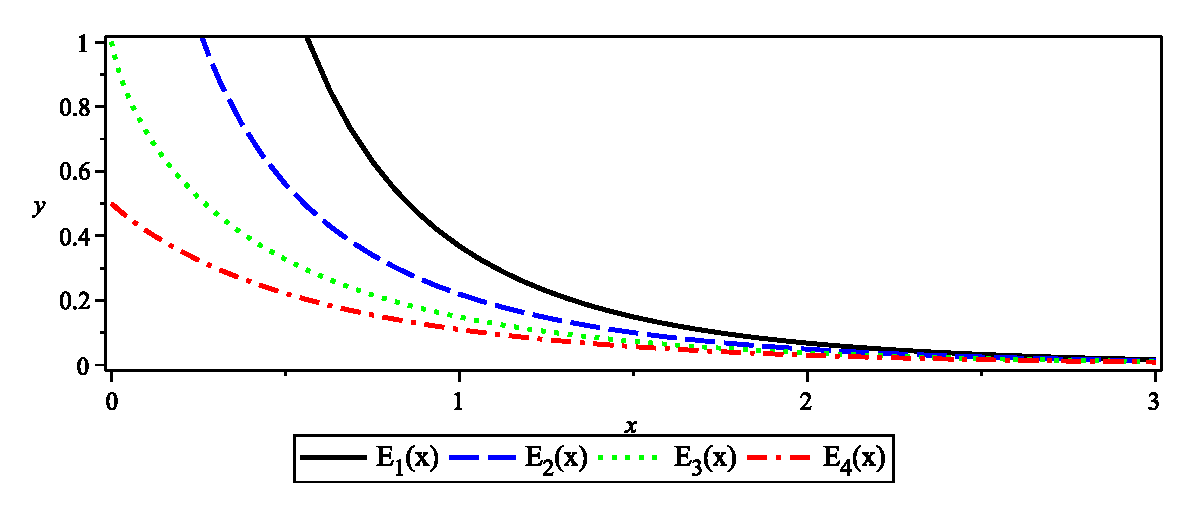
\includegraphics[keepaspectratio, width = 5.0 in]{images/slab_example_exp_functions}
    \caption{The first four exponential functions.}
    \label{fig:slab_example_exp_functions}
\end{figure}

\section*{Further Reading}

The problems discussed in this lecture have been rather elementary in nature.  To explore more realistic problems---even just including scattering in slab geometry---would take us into a much more complicated mathematical domain involving integral transforms (with inverses using complex analysis), singular eigenfunction expansions, and more.  Duderstadt and Martin \cite{duderstadt1976tt} cover most of what has been discussed, and much more.  The motivated student should look to that work (specifically Chapter 2), along with Bell and Glasstone (Chapter 2), Case and Zweifel \cite{case1967ltt}, and Davison \cite{davison1957ntt}.  These are listed in reverse chronological order, and perhaps, in increasing order of difficulty.  Davison in particular uses older notation, so the reader be aware!

\begin{exercises}

  \item \textbf{Cylindrical Coordinates}. Derive the streaming term for the neutron transport equation in 1-d cylindrical geometry.  Include diagrams to help explain your approach.
  
  \item \textbf{Angular Current from Plane Source}. In Example 1, what is the angular current $\mathbf{j}$?

  \item \textbf{Isotropic Current Conditions}. For Example 1, find $\psi$ and $\mathbf{j}$ when the boundary condition is an isotropic angular current (rather than an isotropic angular flux).

  \item \textbf{Flux Inside a Sphere}. Solve for the angular flux on the interior of the spherical shell from Example 2.

  \item \textbf{Angular Redistribution in 1-d}. Explain in your own words why $\psi$ in a 1-d spherical problem depends only on the radius $r$ and cosine of the polar angle $\mu$.  Specifically, why is there no dependence on a second angular variable? 

  \item \textbf{Scalar Flux from Spherical Shell Source}. Solve for the scalar flux on the outside of the sphere in Example 2, i.e. integrate Eq. \ref{eq:spherepsi} over $\mu$.  What happens at $r = r_s$ and why?  What is the limiting behavior of $\phi(r)$ as $r\to \infty$?  In other words, what does the spherical source ``look like'' far from its surface?

  \item \textbf{Current Density in a Slab}. Derive an expression for the current density $\mathbf{J}$ for a purely absorbing slab.  Using the values from the example, generate the curves in Figure \ref{fig:slab_example_phi_current}.  Compute the total absorption rate in the slab and the leakage rate at the boundaries.  Is it what you expect?

\end{exercises}
